\hypertarget{bitSet_8c}{
\section{bit\-Set.c File Reference}
\label{bitSet_8c}\index{bitSet.c@{bitSet.c}}
}
{\tt \#include \char`\"{}errno.h\char`\"{}}\par
{\tt \#include \char`\"{}bit\-Set.h\char`\"{}}\par


Include dependency graph for bit\-Set.c:\begin{figure}[H]
\begin{center}
\leavevmode
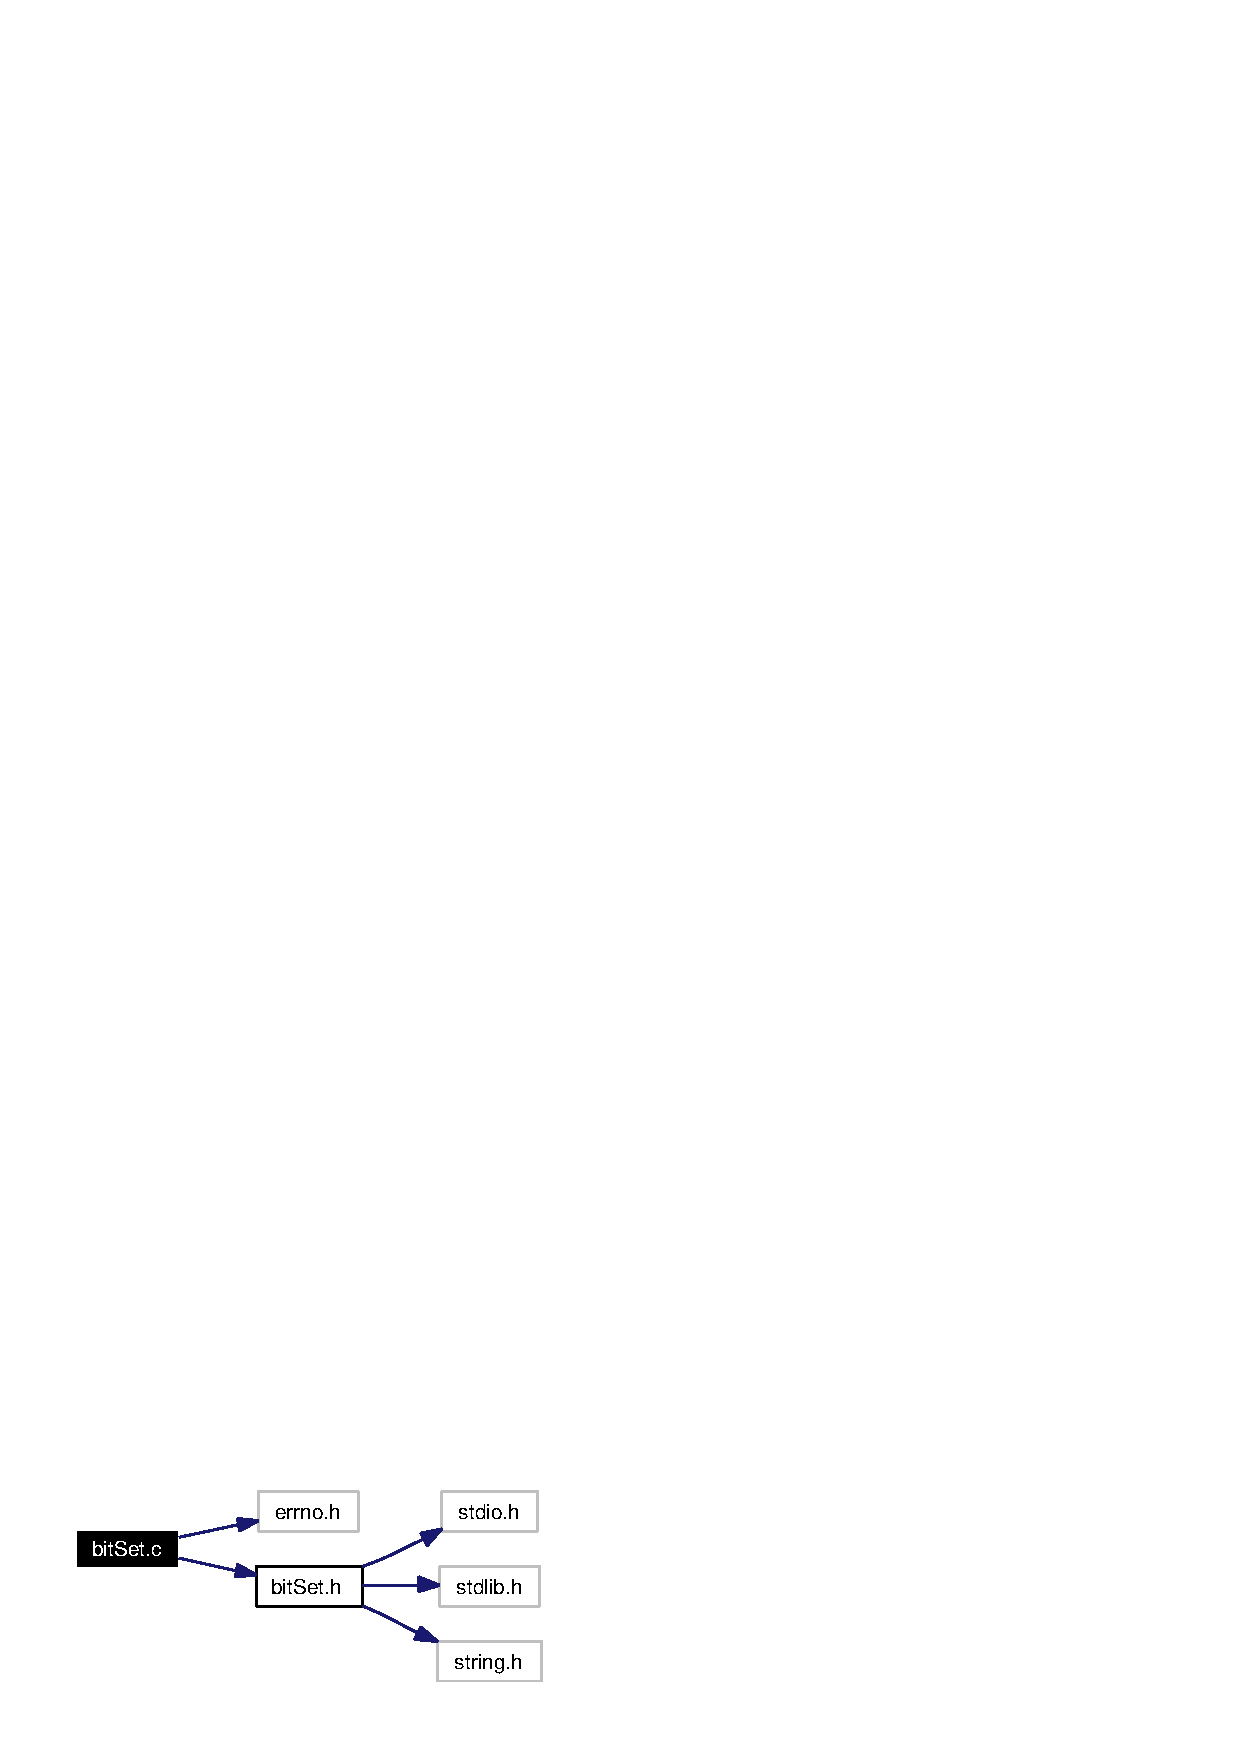
\includegraphics[width=130pt]{bitSet_8c__incl}
\end{center}
\end{figure}
\subsection*{Functions}
\begin{CompactItemize}
\item 
\hyperlink{bitSet_8h_a9}{bit\_\-t} $\ast$ \hyperlink{bitSet_8c_a1}{new\-Bit\-Array} (int bytes)
\item 
\hyperlink{structbitSet__t}{bit\-Set\_\-t} $\ast$ \hyperlink{bitSet_8c_a2}{new\-Bit\-Set} (int size)
\item 
int \hyperlink{bitSet_8c_a3}{set\-True} (\hyperlink{structbitSet__t}{bit\-Set\_\-t} $\ast$s1, int x)
\item 
int \hyperlink{bitSet_8c_a4}{set\-False} (\hyperlink{structbitSet__t}{bit\-Set\_\-t} $\ast$s1, int x)
\item 
int \hyperlink{bitSet_8c_a5}{flip\-Bits} (\hyperlink{structbitSet__t}{bit\-Set\_\-t} $\ast$s1)
\item 
int \hyperlink{bitSet_8c_a6}{fill\-Set} (\hyperlink{structbitSet__t}{bit\-Set\_\-t} $\ast$s1)
\item 
int \hyperlink{bitSet_8c_a7}{empty\-Set} (\hyperlink{structbitSet__t}{bit\-Set\_\-t} $\ast$s1)
\item 
int \hyperlink{bitSet_8c_a8}{check\-Bit} (\hyperlink{structbitSet__t}{bit\-Set\_\-t} $\ast$s1, int x)
\item 
int \hyperlink{bitSet_8c_a9}{delete\-Bit\-Set} (\hyperlink{structbitSet__t}{bit\-Set\_\-t} $\ast$s1)
\item 
int \hyperlink{bitSet_8c_a10}{bit\-Set\-Union} (\hyperlink{structbitSet__t}{bit\-Set\_\-t} $\ast$s1, \hyperlink{structbitSet__t}{bit\-Set\_\-t} $\ast$s2, \hyperlink{structbitSet__t}{bit\-Set\_\-t} $\ast$s3)
\item 
int \hyperlink{bitSet_8c_a11}{copy\-Set} (\hyperlink{structbitSet__t}{bit\-Set\_\-t} $\ast$s1, \hyperlink{structbitSet__t}{bit\-Set\_\-t} $\ast$s2)
\item 
int \hyperlink{bitSet_8c_a12}{copy\-Bit\-Graph} (\hyperlink{structbitGraph__t}{bit\-Graph\_\-t} $\ast$bg1, \hyperlink{structbitGraph__t}{bit\-Graph\_\-t} $\ast$bg2)
\item 
int \hyperlink{bitSet_8c_a13}{bit\-Set\-Difference} (\hyperlink{structbitSet__t}{bit\-Set\_\-t} $\ast$s1, \hyperlink{structbitSet__t}{bit\-Set\_\-t} $\ast$s2, \hyperlink{structbitSet__t}{bit\-Set\_\-t} $\ast$s3)
\item 
int \hyperlink{bitSet_8c_a14}{bit\-Set\-Sum} (\hyperlink{structbitSet__t}{bit\-Set\_\-t} $\ast$s1, \hyperlink{structbitSet__t}{bit\-Set\_\-t} $\ast$s2, \hyperlink{structbitSet__t}{bit\-Set\_\-t} $\ast$s3)
\item 
int \hyperlink{bitSet_8c_a15}{bit\-Set\-Intersection} (\hyperlink{structbitSet__t}{bit\-Set\_\-t} $\ast$s1, \hyperlink{structbitSet__t}{bit\-Set\_\-t} $\ast$s2, \hyperlink{structbitSet__t}{bit\-Set\_\-t} $\ast$s3)
\item 
int \hyperlink{bitSet_8c_a16}{bit\-Set3Way\-Intersection} (\hyperlink{structbitSet__t}{bit\-Set\_\-t} $\ast$s1, \hyperlink{structbitSet__t}{bit\-Set\_\-t} $\ast$s2, \hyperlink{structbitSet__t}{bit\-Set\_\-t} $\ast$s3, \hyperlink{structbitSet__t}{bit\-Set\_\-t} $\ast$s4)
\item 
int \hyperlink{bitSet_8c_a17}{bitcount32} (unsigned int n)
\item 
int \hyperlink{bitSet_8c_a18}{bitcount32\_\-precomp} (unsigned int n)
\item 
int \hyperlink{bitSet_8c_a19}{bitcount64} (unsigned int n)
\item 
int \hyperlink{bitSet_8c_a20}{count\-Set} (\hyperlink{structbitSet__t}{bit\-Set\_\-t} $\ast$s1)
\item 
int \hyperlink{bitSet_8c_a21}{next\-Bit\-Bit\-Set} (\hyperlink{structbitSet__t}{bit\-Set\_\-t} $\ast$s1, int start)
\item 
int \hyperlink{bitSet_8c_a22}{count\-Bit\-Graph\-Non\-Zero} (\hyperlink{structbitGraph__t}{bit\-Graph\_\-t} $\ast$bg)
\item 
int \hyperlink{bitSet_8c_a23}{print\-Bit\-Set} (\hyperlink{structbitSet__t}{bit\-Set\_\-t} $\ast$s1)
\item 
int \hyperlink{bitSet_8c_a24}{bit\-Graph\-Row\-Union} (\hyperlink{structbitGraph__t}{bit\-Graph\_\-t} $\ast$bg, int row1, int row2, \hyperlink{structbitSet__t}{bit\-Set\_\-t} $\ast$s1)
\item 
int \hyperlink{bitSet_8c_a25}{bit\-Graph\-Row\-Intersection} (\hyperlink{structbitGraph__t}{bit\-Graph\_\-t} $\ast$bg, int row1, int row2, \hyperlink{structbitSet__t}{bit\-Set\_\-t} $\ast$s1)
\item 
int \hyperlink{bitSet_8c_a26}{print\-Binary\-Bit\-Set} (\hyperlink{structbitSet__t}{bit\-Set\_\-t} $\ast$s1)
\item 
int \hyperlink{bitSet_8c_a27}{bit\-Graph\-Check\-Bit} (\hyperlink{structbitGraph__t}{bit\-Graph\_\-t} $\ast$bg, int x, int y)
\item 
int \hyperlink{bitSet_8c_a28}{bit\-Graph\-Set\-True} (\hyperlink{structbitGraph__t}{bit\-Graph\_\-t} $\ast$bg, int x, int y)
\item 
int \hyperlink{bitSet_8c_a29}{bit\-Graph\-Set\-False} (\hyperlink{structbitGraph__t}{bit\-Graph\_\-t} $\ast$bg, int x, int y)
\item 
int \hyperlink{bitSet_8c_a30}{bit\-Graph\-Set\-False\-Sym} (\hyperlink{structbitGraph__t}{bit\-Graph\_\-t} $\ast$bg, int x, int y)
\item 
int \hyperlink{bitSet_8c_a31}{bit\-Graph\-Set\-True\-Sym} (\hyperlink{structbitGraph__t}{bit\-Graph\_\-t} $\ast$bg, int x, int y)
\item 
int \hyperlink{bitSet_8c_a32}{bit\-Graph\-Set\-True\-Diagonal} (\hyperlink{structbitGraph__t}{bit\-Graph\_\-t} $\ast$bg)
\item 
int \hyperlink{bitSet_8c_a33}{bit\-Graph\-Set\-False\-Diagonal} (\hyperlink{structbitGraph__t}{bit\-Graph\_\-t} $\ast$bg)
\item 
int \hyperlink{bitSet_8c_a34}{print\-Bit\-Graph} (\hyperlink{structbitGraph__t}{bit\-Graph\_\-t} $\ast$bg)
\item 
int \hyperlink{bitSet_8c_a35}{mask\-Bit\-Graph} (\hyperlink{structbitGraph__t}{bit\-Graph\_\-t} $\ast$bg1, \hyperlink{structbitSet__t}{bit\-Set\_\-t} $\ast$bs)
\item 
int \hyperlink{bitSet_8c_a36}{fill\-Bit\-Graph} (\hyperlink{structbitGraph__t}{bit\-Graph\_\-t} $\ast$bg1)
\item 
int \hyperlink{bitSet_8c_a37}{empty\-Bit\-Graph} (\hyperlink{structbitGraph__t}{bit\-Graph\_\-t} $\ast$bg1)
\item 
\hyperlink{structbitGraph__t}{bit\-Graph\_\-t} $\ast$ \hyperlink{bitSet_8c_a38}{new\-Bit\-Graph} (int size)
\item 
int \hyperlink{bitSet_8c_a39}{empty\-Bit\-Graph\-Row} (\hyperlink{structbitGraph__t}{bit\-Graph\_\-t} $\ast$bg, int row)
\item 
int \hyperlink{bitSet_8c_a40}{delete\-Bit\-Graph} (\hyperlink{structbitGraph__t}{bit\-Graph\_\-t} $\ast$bg)
\end{CompactItemize}


\subsection*{Detailed Description}
This file defines functions for handling bit sets and bit graphs.

Definition in file \hyperlink{bitSet_8c-source}{bit\-Set.c}.

\subsection*{Function Documentation}
\hypertarget{bitSet_8c_a17}{
\index{bitSet.c@{bit\-Set.c}!bitcount32@{bitcount32}}
\index{bitcount32@{bitcount32}!bitSet.c@{bit\-Set.c}}
\subsubsection[bitcount32]{\setlength{\rightskip}{0pt plus 5cm}int bitcount32 (unsigned int {\em n})}}
\label{bitSet_8c_a17}


Attempt at a fast way of counting how many true values are in a given \hyperlink{structbitSet__t}{bit\-Set\_\-t}. Currently deprecated, using precompiled version instead.

Definition at line 351 of file bit\-Set.c.

\scriptsize\begin{verbatim}352 {
353   /*
354      works for 32-bit numbers only 
355    */
356   /*
357      fix last line for 64-bit numbers 
358    */
359 
360   register unsigned int tmp;
361 
362   tmp = n - ((n >> 1) & 033333333333) - ((n >> 2) & 011111111111);
363   return ((tmp + (tmp >> 3)) & 030707070707) % 63;
364 }
\end{verbatim}
\normalsize 


\hypertarget{bitSet_8c_a18}{
\index{bitSet.c@{bit\-Set.c}!bitcount32_precomp@{bitcount32\_\-precomp}}
\index{bitcount32_precomp@{bitcount32\_\-precomp}!bitSet.c@{bit\-Set.c}}
\subsubsection[bitcount32\_\-precomp]{\setlength{\rightskip}{0pt plus 5cm}int bitcount32\_\-precomp (unsigned int {\em n})}}
\label{bitSet_8c_a18}


Uses bits\_\-in\_\-char data structure to determine the number of true bits in a 32-bit int in an efficient manner. Input: 32-bit int (equal to one slot in the bit\-Set). Output: number of true bits in the input integer.

Definition at line 396 of file bit\-Set.c.

Referenced by count\-Set().

\scriptsize\begin{verbatim}397 {
398   // works only for 32-bit ints
399 
400   return bits_in_char[n & 0xffu]
401     + bits_in_char[(n >> 8) & 0xffu]
402     + bits_in_char[(n >> 16) & 0xffu] + bits_in_char[(n >> 24) & 0xffu];
403 }
\end{verbatim}
\normalsize 


\hypertarget{bitSet_8c_a19}{
\index{bitSet.c@{bit\-Set.c}!bitcount64@{bitcount64}}
\index{bitcount64@{bitcount64}!bitSet.c@{bit\-Set.c}}
\subsubsection[bitcount64]{\setlength{\rightskip}{0pt plus 5cm}int bitcount64 (unsigned int {\em n})}}
\label{bitSet_8c_a19}


Currently there is no support for 64-bit architectures.

Definition at line 420 of file bit\-Set.c.

\scriptsize\begin{verbatim}421 {
422   n = PCCOUNT (n, 0);
423   n = PCCOUNT (n, 1);
424   n = PCCOUNT (n, 2);
425   n = PCCOUNT (n, 3);
426   n = PCCOUNT (n, 4);
427   n = PCCOUNT (n, 5);       // for 64-bit integers 
428   return n;
429 }
\end{verbatim}
\normalsize 


\hypertarget{bitSet_8c_a27}{
\index{bitSet.c@{bit\-Set.c}!bitGraphCheckBit@{bitGraphCheckBit}}
\index{bitGraphCheckBit@{bitGraphCheckBit}!bitSet.c@{bit\-Set.c}}
\subsubsection[bitGraphCheckBit]{\setlength{\rightskip}{0pt plus 5cm}int bit\-Graph\-Check\-Bit (\hyperlink{structbitGraph__t}{bit\-Graph\_\-t} $\ast$ {\em bg}, int {\em x}, int {\em y})}}
\label{bitSet_8c_a27}


Checks the value of a bit in a \hyperlink{structbitGraph__t}{bit\-Graph\_\-t} object. Input: a \hyperlink{structbitGraph__t}{bit\-Graph\_\-t} object, the index of the row of the \hyperlink{structbitGraph__t}{bit\-Graph\_\-t} with the bit to be checked, the index of the bit in that row that is to be checked. Output: the value of the bit in the bit\-Graph being checked.

Definition at line 628 of file bit\-Set.c.

References check\-Bit(), and bit\-Graph\_\-t::graph.

Referenced by main(), and measure\-Diagonal().

\scriptsize\begin{verbatim}629 {
630   return checkBit (bg->graph[x], y);
631 }
\end{verbatim}
\normalsize 


\hypertarget{bitSet_8c_a25}{
\index{bitSet.c@{bit\-Set.c}!bitGraphRowIntersection@{bitGraphRowIntersection}}
\index{bitGraphRowIntersection@{bitGraphRowIntersection}!bitSet.c@{bit\-Set.c}}
\subsubsection[bitGraphRowIntersection]{\setlength{\rightskip}{0pt plus 5cm}int bit\-Graph\-Row\-Intersection (\hyperlink{structbitGraph__t}{bit\-Graph\_\-t} $\ast$ {\em bg}, int {\em row1}, int {\em row2}, \hyperlink{structbitSet__t}{bit\-Set\_\-t} $\ast$ {\em s1})}}
\label{bitSet_8c_a25}


Finds the intersection of two rows (bit\-Sets) within a \hyperlink{structbitGraph__t}{bit\-Graph\_\-t} object. Input: a \hyperlink{structbitGraph__t}{bit\-Graph\_\-t} object, first row to be compared, second row to be compared, and a \hyperlink{structbitSet__t}{bit\-Set\_\-t} to store the intersection results. Output: integer success value of 0 (and an altered destination \hyperlink{structbitSet__t}{bit\-Set\_\-t} object with a true value wherever both source bit\-Sets had a true value).

Definition at line 598 of file bit\-Set.c.

References bit\-Set\-Intersection(), and bit\-Graph\_\-t::graph.

Referenced by get\-Stat\-Mat(), and old\-Get\-Stat\-Mat().

\scriptsize\begin{verbatim}599 {
600   bitSetIntersection (bg->graph[row1], bg->graph[row2], s1);
601   return 0;
602 }
\end{verbatim}
\normalsize 


\hypertarget{bitSet_8c_a24}{
\index{bitSet.c@{bit\-Set.c}!bitGraphRowUnion@{bitGraphRowUnion}}
\index{bitGraphRowUnion@{bitGraphRowUnion}!bitSet.c@{bit\-Set.c}}
\subsubsection[bitGraphRowUnion]{\setlength{\rightskip}{0pt plus 5cm}int bit\-Graph\-Row\-Union (\hyperlink{structbitGraph__t}{bit\-Graph\_\-t} $\ast$ {\em bg}, int {\em row1}, int {\em row2}, \hyperlink{structbitSet__t}{bit\-Set\_\-t} $\ast$ {\em s1})}}
\label{bitSet_8c_a24}


Finds the union of two rows (bit\-Sets) within a bit\-Graph Input: a \hyperlink{structbitGraph__t}{bit\-Graph\_\-t} object, first row to be compared, second row to be compared, and a \hyperlink{structbitSet__t}{bit\-Set\_\-t} to store the union results. Output: integer success value of 0 (and an altered destination \hyperlink{structbitSet__t}{bit\-Set\_\-t} object with a true value wherever one or both source bit\-Sets had a true value).

Definition at line 584 of file bit\-Set.c.

References bit\-Set\-Union(), and bit\-Graph\_\-t::graph.

\scriptsize\begin{verbatim}585 {
586   bitSetUnion (bg->graph[row1], bg->graph[row2], s1);
587   return 0;
588 }
\end{verbatim}
\normalsize 


\hypertarget{bitSet_8c_a29}{
\index{bitSet.c@{bit\-Set.c}!bitGraphSetFalse@{bitGraphSetFalse}}
\index{bitGraphSetFalse@{bitGraphSetFalse}!bitSet.c@{bit\-Set.c}}
\subsubsection[bitGraphSetFalse]{\setlength{\rightskip}{0pt plus 5cm}int bit\-Graph\-Set\-False (\hyperlink{structbitGraph__t}{bit\-Graph\_\-t} $\ast$ {\em bg}, int {\em x}, int {\em y})}}
\label{bitSet_8c_a29}


Sets a specific bit in a bit\-Graph false. Input: a \hyperlink{structbitGraph__t}{bit\-Graph\_\-t} object, the index of the row of the \hyperlink{structbitGraph__t}{bit\-Graph\_\-t} with the bit be set, the index of the bit in that row that is to be set. Output: integer success value of 0 (and an altered \hyperlink{structbitGraph__t}{bit\-Graph\_\-t} object).

Definition at line 654 of file bit\-Set.c.

References bit\-Graph\_\-t::graph, and set\-False().

\scriptsize\begin{verbatim}655 {
656   setFalse (bg->graph[x], y);
657   return 0;
658 }
\end{verbatim}
\normalsize 


\hypertarget{bitSet_8c_a33}{
\index{bitSet.c@{bit\-Set.c}!bitGraphSetFalseDiagonal@{bitGraphSetFalseDiagonal}}
\index{bitGraphSetFalseDiagonal@{bitGraphSetFalseDiagonal}!bitSet.c@{bit\-Set.c}}
\subsubsection[bitGraphSetFalseDiagonal]{\setlength{\rightskip}{0pt plus 5cm}int bit\-Graph\-Set\-False\-Diagonal (\hyperlink{structbitGraph__t}{bit\-Graph\_\-t} $\ast$ {\em bg})}}
\label{bitSet_8c_a33}


Sets the main diagonal of a bit\-Graph false. Input: a \hyperlink{structbitGraph__t}{bit\-Graph\_\-t} object. Output: integer success value of 0 (and an altered \hyperlink{structbitGraph__t}{bit\-Graph\_\-t} object).

Definition at line 714 of file bit\-Set.c.

References bit\-Graph\_\-t::graph, and set\-False().

Referenced by convolve().

\scriptsize\begin{verbatim}715 {
716   int i;
717   for (i = 0; i < bg->size; i++)
718     {
719       setFalse (bg->graph[i], i);
720     }
721   return 0;
722 }
\end{verbatim}
\normalsize 


\hypertarget{bitSet_8c_a30}{
\index{bitSet.c@{bit\-Set.c}!bitGraphSetFalseSym@{bitGraphSetFalseSym}}
\index{bitGraphSetFalseSym@{bitGraphSetFalseSym}!bitSet.c@{bit\-Set.c}}
\subsubsection[bitGraphSetFalseSym]{\setlength{\rightskip}{0pt plus 5cm}int bit\-Graph\-Set\-False\-Sym (\hyperlink{structbitGraph__t}{bit\-Graph\_\-t} $\ast$ {\em bg}, int {\em x}, int {\em y})}}
\label{bitSet_8c_a30}


Sets a specific bit and its symmetric opposite in a bit\-Graph false. For instance, given that we wanted to set the 3rd bit in the 5th row false, this would also set the 5th bit in the 3rd row. Input: a \hyperlink{structbitGraph__t}{bit\-Graph\_\-t} object, the index of the row of the bit\-Graph with the bit be set, the index of the bit in that row that is to be set. Output: integer success value of 0 (and an altered \hyperlink{structbitGraph__t}{bit\-Graph\_\-t} object).

Definition at line 669 of file bit\-Set.c.

References bit\-Graph\_\-t::graph, and set\-False().

\scriptsize\begin{verbatim}670 {
671   setFalse (bg->graph[x], y);
672   setFalse (bg->graph[y], x);
673   return 0;
674 }
\end{verbatim}
\normalsize 


\hypertarget{bitSet_8c_a28}{
\index{bitSet.c@{bit\-Set.c}!bitGraphSetTrue@{bitGraphSetTrue}}
\index{bitGraphSetTrue@{bitGraphSetTrue}!bitSet.c@{bit\-Set.c}}
\subsubsection[bitGraphSetTrue]{\setlength{\rightskip}{0pt plus 5cm}int bit\-Graph\-Set\-True (\hyperlink{structbitGraph__t}{bit\-Graph\_\-t} $\ast$ {\em bg}, int {\em x}, int {\em y})}}
\label{bitSet_8c_a28}


Sets a specific bit in a bit\-Graph true. Input: a \hyperlink{structbitGraph__t}{bit\-Graph\_\-t} object, the index of the row of the \hyperlink{structbitGraph__t}{bit\-Graph\_\-t} with the bit be set, the index of the bit in that row that is to be set. Output: integer success value of 0 (and an altered \hyperlink{structbitGraph__t}{bit\-Graph\_\-t} object).

Definition at line 641 of file bit\-Set.c.

References bit\-Graph\_\-t::graph, and set\-True().

\scriptsize\begin{verbatim}642 {
643   setTrue (bg->graph[x], y);
644   return 0;
645 }
\end{verbatim}
\normalsize 


\hypertarget{bitSet_8c_a32}{
\index{bitSet.c@{bit\-Set.c}!bitGraphSetTrueDiagonal@{bitGraphSetTrueDiagonal}}
\index{bitGraphSetTrueDiagonal@{bitGraphSetTrueDiagonal}!bitSet.c@{bit\-Set.c}}
\subsubsection[bitGraphSetTrueDiagonal]{\setlength{\rightskip}{0pt plus 5cm}int bit\-Graph\-Set\-True\-Diagonal (\hyperlink{structbitGraph__t}{bit\-Graph\_\-t} $\ast$ {\em bg})}}
\label{bitSet_8c_a32}


Sets the main diagonal of a bit\-Graph true. Input: a \hyperlink{structbitGraph__t}{bit\-Graph\_\-t} object. Output: integer success value of 0 (and an altered \hyperlink{structbitGraph__t}{bit\-Graph\_\-t} object).

Definition at line 698 of file bit\-Set.c.

References bit\-Graph\_\-t::graph, and set\-True().

\scriptsize\begin{verbatim}699 {
700   int i;
701   for (i = 0; i < bg->size; i++)
702     {
703       setTrue (bg->graph[i], i);
704     }
705   return 0;
706 }
\end{verbatim}
\normalsize 


\hypertarget{bitSet_8c_a31}{
\index{bitSet.c@{bit\-Set.c}!bitGraphSetTrueSym@{bitGraphSetTrueSym}}
\index{bitGraphSetTrueSym@{bitGraphSetTrueSym}!bitSet.c@{bit\-Set.c}}
\subsubsection[bitGraphSetTrueSym]{\setlength{\rightskip}{0pt plus 5cm}int bit\-Graph\-Set\-True\-Sym (\hyperlink{structbitGraph__t}{bit\-Graph\_\-t} $\ast$ {\em bg}, int {\em x}, int {\em y})}}
\label{bitSet_8c_a31}


Sets a specific bit and its symmetric opposite in a bit\-Graph true. For instance, given that we wanted to set the 3rd bit in the 5th row true, this would also set the 5th bit in the 3rd row. Input: a bit\-Graph, the index of the row of the bit\-Graph with the bit be set, the index of the bit in that row that is to be set. Output: integer success value of 0 (and an altered \hyperlink{structbitGraph__t}{bit\-Graph\_\-t} object).

Definition at line 685 of file bit\-Set.c.

References bit\-Graph\_\-t::graph, and set\-True().

Referenced by align\-Words\-Mat\_\-bit(), main(), and real\-Comparison().

\scriptsize\begin{verbatim}686 {
687   setTrue (bg->graph[x], y);
688   setTrue (bg->graph[y], x);
689   return 0;
690 }
\end{verbatim}
\normalsize 


\hypertarget{bitSet_8c_a16}{
\index{bitSet.c@{bit\-Set.c}!bitSet3WayIntersection@{bitSet3WayIntersection}}
\index{bitSet3WayIntersection@{bitSet3WayIntersection}!bitSet.c@{bit\-Set.c}}
\subsubsection[bitSet3WayIntersection]{\setlength{\rightskip}{0pt plus 5cm}int bit\-Set3Way\-Intersection (\hyperlink{structbitSet__t}{bit\-Set\_\-t} $\ast$ {\em s1}, \hyperlink{structbitSet__t}{bit\-Set\_\-t} $\ast$ {\em s2}, \hyperlink{structbitSet__t}{bit\-Set\_\-t} $\ast$ {\em s3}, \hyperlink{structbitSet__t}{bit\-Set\_\-t} $\ast$ {\em s4})}}
\label{bitSet_8c_a16}


Finds the intersection of 3 bit\-Sets. Input: First bit\-Set to be intersected, second bitset to be intersected. third bit\-Set to be intersected, a bit\-Set to store the result of the intersection. Output: Integer success value of 0 (and an altered destination \hyperlink{structbitSet__t}{bit\-Set\_\-t} object with a true where all three source bit\-Sets had a true.)

Definition at line 327 of file bit\-Set.c.

References BSINTERSECTION, bit\-Set\_\-t::slots, and bit\-Set\_\-t::tf.

\scriptsize\begin{verbatim}329 {
330   int i;
331   if ((s1->slots != s2->slots) || (s1->slots != s3->slots)
332       || (s1->slots != s4->slots))
333     {
334       fprintf (stderr, "Sets aren't same size!\n");
335       fflush (stderr);
336       exit (0);
337     }
338   for (i = 0; i < s1->slots; i++)
339     {
340       s4->tf[i] = BSINTERSECTION (s1->tf[i], s2->tf[i]);
341       s4->tf[i] = BSINTERSECTION (s3->tf[i], s4->tf[i]);
342     }
343   return 0;
344 }
\end{verbatim}
\normalsize 


\hypertarget{bitSet_8c_a13}{
\index{bitSet.c@{bit\-Set.c}!bitSetDifference@{bitSetDifference}}
\index{bitSetDifference@{bitSetDifference}!bitSet.c@{bit\-Set.c}}
\subsubsection[bitSetDifference]{\setlength{\rightskip}{0pt plus 5cm}int bit\-Set\-Difference (\hyperlink{structbitSet__t}{bit\-Set\_\-t} $\ast$ {\em s1}, \hyperlink{structbitSet__t}{bit\-Set\_\-t} $\ast$ {\em s2}, \hyperlink{structbitSet__t}{bit\-Set\_\-t} $\ast$ {\em s3})}}
\label{bitSet_8c_a13}


Locates all differences between two bit\-Sets. The result bit\-Set contains a true at a given bit if the two source bit\-Sets differ at that bit. Input: first bit set to be compared, second bit set to be compared. third bit set to store the results Output: integer success value of 0 (and an altered destination \hyperlink{structbitSet__t}{bit\-Set\_\-t} object with a true where the two source bit sets differed).

Definition at line 254 of file bit\-Set.c.

References bit\-Set\_\-t::slots, and bit\-Set\_\-t::tf.

\scriptsize\begin{verbatim}255 {
256   int i;
257   if ((s1->slots != s2->slots) || (s1->slots != s3->slots))
258     {
259       fprintf (stderr, "Sets aren't same size!\n");
260       fflush (stderr);
261       exit (0);
262     }
263   for (i = 0; i < s1->slots; i++)
264     {
265       s3->tf[i] = (s1->tf[i] & (~s2->tf[i]));
266     }
267   return 0;
268 }
\end{verbatim}
\normalsize 


\hypertarget{bitSet_8c_a15}{
\index{bitSet.c@{bit\-Set.c}!bitSetIntersection@{bitSetIntersection}}
\index{bitSetIntersection@{bitSetIntersection}!bitSet.c@{bit\-Set.c}}
\subsubsection[bitSetIntersection]{\setlength{\rightskip}{0pt plus 5cm}int bit\-Set\-Intersection (\hyperlink{structbitSet__t}{bit\-Set\_\-t} $\ast$ {\em s1}, \hyperlink{structbitSet__t}{bit\-Set\_\-t} $\ast$ {\em s2}, \hyperlink{structbitSet__t}{bit\-Set\_\-t} $\ast$ {\em s3})}}
\label{bitSet_8c_a15}


Finds the intersection of two bitsets. Input: First bit\-Set to be intersected, second bit\-Set to be intersected. a bit\-Set to store the result of the intersection. Output: Integer success value of 0 (and an altered destination \hyperlink{structbitSet__t}{bit\-Set\_\-t} object. with a true where both source bit\-Sets had a true).

Definition at line 299 of file bit\-Set.c.

References BSINTERSECTION, bit\-Set\_\-t::slots, and bit\-Set\_\-t::tf.

Referenced by bit\-Graph\-Row\-Intersection(), find\-Cliques(), and mask\-Bit\-Graph().

\scriptsize\begin{verbatim}300 {
301   int i;
302   if ((s1->slots != s2->slots) || (s1->slots != s3->slots))
303     {
304       fprintf (stderr, "Sets aren't same size!\n");
305       fprintf (stderr, "set 1 slots = %d\n", s1->slots);
306       fprintf (stderr, "set 2 slots = %d\n", s2->slots);
307       fprintf (stderr, "set 3 slots = %d\n", s3->slots);
308       fflush (stderr);
309       exit (0);
310     }
311   for (i = 0; i < s1->slots; i++)
312     {
313       s3->tf[i] = BSINTERSECTION (s1->tf[i], s2->tf[i]);
314     }
315   return 0;
316 }
\end{verbatim}
\normalsize 


\hypertarget{bitSet_8c_a14}{
\index{bitSet.c@{bit\-Set.c}!bitSetSum@{bitSetSum}}
\index{bitSetSum@{bitSetSum}!bitSet.c@{bit\-Set.c}}
\subsubsection[bitSetSum]{\setlength{\rightskip}{0pt plus 5cm}int bit\-Set\-Sum (\hyperlink{structbitSet__t}{bit\-Set\_\-t} $\ast$ {\em s1}, \hyperlink{structbitSet__t}{bit\-Set\_\-t} $\ast$ {\em s2}, \hyperlink{structbitSet__t}{bit\-Set\_\-t} $\ast$ {\em s3})}}
\label{bitSet_8c_a14}


Adds two \hyperlink{structbitSet__t}{bit\-Set\_\-t} objects together. Currently unknown functionality, not used in existing code.

Definition at line 275 of file bit\-Set.c.

References bit\-Set\_\-t::slots, and bit\-Set\_\-t::tf.

\scriptsize\begin{verbatim}276 {
277   int i;
278   if ((s1->slots != s2->slots) || (s1->slots != s3->slots))
279     {
280       fprintf (stderr, "Sets aren't same size!\n");
281       fflush (stderr);
282       exit (0);
283     }
284   for (i = 0; i < s1->slots; i++)
285     {
286       s3->tf[i] = (s1->tf[i] + s2->tf[i]);
287     }
288   return 0;
289 }
\end{verbatim}
\normalsize 


\hypertarget{bitSet_8c_a10}{
\index{bitSet.c@{bit\-Set.c}!bitSetUnion@{bitSetUnion}}
\index{bitSetUnion@{bitSetUnion}!bitSet.c@{bit\-Set.c}}
\subsubsection[bitSetUnion]{\setlength{\rightskip}{0pt plus 5cm}int bit\-Set\-Union (\hyperlink{structbitSet__t}{bit\-Set\_\-t} $\ast$ {\em s1}, \hyperlink{structbitSet__t}{bit\-Set\_\-t} $\ast$ {\em s2}, \hyperlink{structbitSet__t}{bit\-Set\_\-t} $\ast$ {\em s3})}}
\label{bitSet_8c_a10}


Finds the union of two bit\-Sets Input: first bit set for the union, second bit set for the union. a bit set in which to store the results Output: an integer success value of 0 (and an altered third \hyperlink{structbitSet__t}{bit\-Set\_\-t} with the results of the union.

Definition at line 182 of file bit\-Set.c.

References BSUNION, bit\-Set\_\-t::slots, and bit\-Set\_\-t::tf.

Referenced by bit\-Graph\-Row\-Union(), and single\-Linkage().

\scriptsize\begin{verbatim}183 {
184   int i;
185   if ((s1->slots != s2->slots) || (s1->slots != s3->slots))
186     {
187       fprintf (stderr, "Sets aren't same size!\n");
188       fflush (stderr);
189       exit (0);
190     }
191   for (i = 0; i < s1->slots; i++)
192     {
193       s3->tf[i] = BSUNION (s1->tf[i], s2->tf[i]);
194     }
195   return 0;
196 }
\end{verbatim}
\normalsize 


\hypertarget{bitSet_8c_a8}{
\index{bitSet.c@{bit\-Set.c}!checkBit@{checkBit}}
\index{checkBit@{checkBit}!bitSet.c@{bit\-Set.c}}
\subsubsection[checkBit]{\setlength{\rightskip}{0pt plus 5cm}int check\-Bit (\hyperlink{structbitSet__t}{bit\-Set\_\-t} $\ast$ {\em s1}, int {\em x})}}
\label{bitSet_8c_a8}


Finds the value of a specific bit in a bit\-Set. Input: a bit\-Set, the number of the bit being queried. Output: the value of the bit being queried (1 or 0).

Definition at line 148 of file bit\-Set.c.

References BSTEST, and bit\-Set\_\-t::tf.

Referenced by bit\-Graph\-Check\-Bit(), find\-Cliques(), get\-Stat\-Mat(), mask\-Bit\-Graph(), next\-Bit\-Bit\-Set(), single\-Linkage(), and whole\-Round\-Conv().

\scriptsize\begin{verbatim}149 {
150   return BSTEST (s1->tf, x);
151 }
\end{verbatim}
\normalsize 


\hypertarget{bitSet_8c_a12}{
\index{bitSet.c@{bit\-Set.c}!copyBitGraph@{copyBitGraph}}
\index{copyBitGraph@{copyBitGraph}!bitSet.c@{bit\-Set.c}}
\subsubsection[copyBitGraph]{\setlength{\rightskip}{0pt plus 5cm}int copy\-Bit\-Graph (\hyperlink{structbitGraph__t}{bit\-Graph\_\-t} $\ast$ {\em bg1}, \hyperlink{structbitGraph__t}{bit\-Graph\_\-t} $\ast$ {\em bg2})}}
\label{bitSet_8c_a12}


Copies the true/false contents of one bit graph into an existing bit graph. Both bit graphs must be the same size, and each corresponding bit set between the two bit graphs must be the same size. Input: source bit graph, destination \hyperlink{structbitGraph__t}{bit\-Graph\_\-t} object. Output: integer success value of 0 (and an altered destination bit graph).

Definition at line 229 of file bit\-Set.c.

References copy\-Set(), bit\-Graph\_\-t::graph, and bit\-Graph\_\-t::size.

\scriptsize\begin{verbatim}230 {
231   int i;
232   if (bg1->size != bg2->size)
233     {
234       fprintf (stderr, "Graphs are not the same size!");
235       fflush (stderr);
236       exit (0);
237     }
238   for (i = 0; i < bg1->size; i++)
239     {
240       copySet (bg1->graph[i], bg2->graph[i]);
241     }
242   return 0;
243 }
\end{verbatim}
\normalsize 


\hypertarget{bitSet_8c_a11}{
\index{bitSet.c@{bit\-Set.c}!copySet@{copySet}}
\index{copySet@{copySet}!bitSet.c@{bit\-Set.c}}
\subsubsection[copySet]{\setlength{\rightskip}{0pt plus 5cm}int copy\-Set (\hyperlink{structbitSet__t}{bit\-Set\_\-t} $\ast$ {\em s1}, \hyperlink{structbitSet__t}{bit\-Set\_\-t} $\ast$ {\em s2})}}
\label{bitSet_8c_a11}


Copies the true/false contents of one bit set into an existing bit set. Both bit sets must be the same size. Input: source bit set, destination \hyperlink{structbitSet__t}{bit\-Set\_\-t} object. Output: integer success value of 0 (and an altered destination bitset.

Definition at line 205 of file bit\-Set.c.

References bit\-Set\_\-t::slots, and bit\-Set\_\-t::tf.

Referenced by copy\-Bit\-Graph(), filter\-Graph(), and single\-Linkage().

\scriptsize\begin{verbatim}206 {
207   int i;
208   if (s1->slots != s2->slots)
209     {
210       fprintf (stderr, "Sets are not the same size!");
211       fflush (stderr);
212       exit (0);
213     }
214   for (i = 0; i < s1->slots; i++)
215     {
216       s2->tf[i] = s1->tf[i];
217     }
218   return 0;
219 }
\end{verbatim}
\normalsize 


\hypertarget{bitSet_8c_a22}{
\index{bitSet.c@{bit\-Set.c}!countBitGraphNonZero@{countBitGraphNonZero}}
\index{countBitGraphNonZero@{countBitGraphNonZero}!bitSet.c@{bit\-Set.c}}
\subsubsection[countBitGraphNonZero]{\setlength{\rightskip}{0pt plus 5cm}int count\-Bit\-Graph\-Non\-Zero (\hyperlink{structbitGraph__t}{bit\-Graph\_\-t} $\ast$ {\em bg})}}
\label{bitSet_8c_a22}


Counts the number of true (non-zero) values in a \hyperlink{structbitGraph__t}{bit\-Graph\_\-t} object. Input: a \hyperlink{structbitGraph__t}{bit\-Graph\_\-t} object. Output: the integer number of true (non-zero) values in the \hyperlink{structbitGraph__t}{bit\-Graph\_\-t} object.

Definition at line 537 of file bit\-Set.c.

References count\-Set(), and bit\-Graph\_\-t::graph.

\scriptsize\begin{verbatim}538 {
539   int i;
540   int sum = 0;
541   // Iterate over all bitSets in the bitGraph
542   for (i = 0; i < bg->size; i++)
543     {
544       sum += countSet (bg->graph[i]);
545     }
546   return sum;
547 }
\end{verbatim}
\normalsize 


\hypertarget{bitSet_8c_a20}{
\index{bitSet.c@{bit\-Set.c}!countSet@{countSet}}
\index{countSet@{countSet}!bitSet.c@{bit\-Set.c}}
\subsubsection[countSet]{\setlength{\rightskip}{0pt plus 5cm}int count\-Set (\hyperlink{structbitSet__t}{bit\-Set\_\-t} $\ast$ {\em s1})}}
\label{bitSet_8c_a20}


Counts the number of true values in a bit\-Set. Input: a \hyperlink{structbitSet__t}{bit\-Set\_\-t} object. Output: number of true values in that \hyperlink{structbitSet__t}{bit\-Set\_\-t} object.

Definition at line 437 of file bit\-Set.c.

References bitcount32\_\-precomp(), and bit\-Set\_\-t::tf.

Referenced by bit\-Set\-To\-CSet(), count\-Bit\-Graph\-Non\-Zero(), filter\-Graph(), filter\-Iter(), find\-Cliques(), get\-Stat\-Mat(), old\-Get\-Stat\-Mat(), print\-Bit\-Set(), single\-Linkage(), and whole\-Clique\-Conv().

\scriptsize\begin{verbatim}438 {
439   int i;
440   int sum = 0;
441   int (*bitCounter) () = &bitcount32_precomp;
442   // Currently there is no support for 64-bit architectures.
443 
444   if (sizeof (bit_t) * 8 != 32)
445     {
446       fprintf (stderr,
447            "\nSorry, no support for 64-bit architectures just yet! - countSet\n");
448       fflush (stderr);
449       exit (0);
450     }
451 
452   // Just count the number of true bits in each char, and do this for
453   // (num of chars per int) chars.
454   for (i = 0; i < s1->slots; i++)
455     {
456       sum += bitCounter (s1->tf[i]);
457     }
458   return sum;
459 }
\end{verbatim}
\normalsize 


\hypertarget{bitSet_8c_a40}{
\index{bitSet.c@{bit\-Set.c}!deleteBitGraph@{deleteBitGraph}}
\index{deleteBitGraph@{deleteBitGraph}!bitSet.c@{bit\-Set.c}}
\subsubsection[deleteBitGraph]{\setlength{\rightskip}{0pt plus 5cm}int delete\-Bit\-Graph (\hyperlink{structbitGraph__t}{bit\-Graph\_\-t} $\ast$ {\em bg})}}
\label{bitSet_8c_a40}


Deletes a \hyperlink{structbitGraph__t}{bit\-Graph\_\-t} object from memory. Input: a \hyperlink{structbitGraph__t}{bit\-Graph\_\-t} object to be deleted. Output: integer success value from 0 (and deletion of a \hyperlink{structbitGraph__t}{bit\-Graph\_\-t} object).

Definition at line 853 of file bit\-Set.c.

References delete\-Bit\-Set(), and bit\-Graph\_\-t::graph.

Referenced by main().

\scriptsize\begin{verbatim}854 {
855   int i;
856   if (bg != NULL)
857     {
858       if (bg->graph != NULL)
859     {
860       for (i = 0; i < bg->size; i++)
861         {
862           deleteBitSet (bg->graph[i]);
863         }
864       free (bg->graph);
865       bg->graph = NULL;
866     }
867       free (bg);
868       bg = NULL;
869     }
870   return 0;
871 }
\end{verbatim}
\normalsize 


\hypertarget{bitSet_8c_a9}{
\index{bitSet.c@{bit\-Set.c}!deleteBitSet@{deleteBitSet}}
\index{deleteBitSet@{deleteBitSet}!bitSet.c@{bit\-Set.c}}
\subsubsection[deleteBitSet]{\setlength{\rightskip}{0pt plus 5cm}int delete\-Bit\-Set (\hyperlink{structbitSet__t}{bit\-Set\_\-t} $\ast$ {\em s1})}}
\label{bitSet_8c_a9}


Performs memory management for the deletion of a \hyperlink{structbitSet__t}{bit\-Set\_\-t} structure. Input: a \hyperlink{structbitSet__t}{bit\-Set\_\-t} object. Output: integer success value of 1.

Definition at line 159 of file bit\-Set.c.

References bit\-Set\_\-t::tf.

Referenced by convolve(), delete\-Bit\-Graph(), filter\-Graph(), find\-Cliques(), get\-Stat\-Mat(), old\-Get\-Stat\-Mat(), whole\-Clique\-Conv(), and whole\-Round\-Conv().

\scriptsize\begin{verbatim}160 {
161   if (s1->tf != NULL)
162     {
163       free (s1->tf);
164       s1->tf = NULL;
165     }
166   if (s1 != NULL)
167     {
168       free (s1);
169       s1 = NULL;
170     }
171   return 0;
172 }
\end{verbatim}
\normalsize 


\hypertarget{bitSet_8c_a37}{
\index{bitSet.c@{bit\-Set.c}!emptyBitGraph@{emptyBitGraph}}
\index{emptyBitGraph@{emptyBitGraph}!bitSet.c@{bit\-Set.c}}
\subsubsection[emptyBitGraph]{\setlength{\rightskip}{0pt plus 5cm}int empty\-Bit\-Graph (\hyperlink{structbitGraph__t}{bit\-Graph\_\-t} $\ast$ {\em bg1})}}
\label{bitSet_8c_a37}


Sets all bits in the \hyperlink{structbitGraph__t}{bit\-Graph\_\-t} object to false. Input: a \hyperlink{structbitGraph__t}{bit\-Graph\_\-t} object. Output: integer success value of 0 (and a \hyperlink{structbitGraph__t}{bit\-Graph\_\-t} with all false bits).

Definition at line 791 of file bit\-Set.c.

References empty\-Set(), and bit\-Graph\_\-t::graph.

\scriptsize\begin{verbatim}792 {
793   int i;
794   for (i = 0; i < bg1->size; i++)
795     {
796       emptySet (bg1->graph[i]);
797     }
798   return 0;
799 }
\end{verbatim}
\normalsize 


\hypertarget{bitSet_8c_a39}{
\index{bitSet.c@{bit\-Set.c}!emptyBitGraphRow@{emptyBitGraphRow}}
\index{emptyBitGraphRow@{emptyBitGraphRow}!bitSet.c@{bit\-Set.c}}
\subsubsection[emptyBitGraphRow]{\setlength{\rightskip}{0pt plus 5cm}int empty\-Bit\-Graph\-Row (\hyperlink{structbitGraph__t}{bit\-Graph\_\-t} $\ast$ {\em bg}, int {\em row})}}
\label{bitSet_8c_a39}


Sets all bits in a \hyperlink{structbitGraph__t}{bit\-Graph\_\-t} row (a \hyperlink{structbitSet__t}{bit\-Set\_\-t} object) false. Input: a bit\-Graph, a row in the \hyperlink{structbitGraph__t}{bit\-Graph\_\-t} object to be emptied. Output: integer success value of 0 (and an altered \hyperlink{structbitGraph__t}{bit\-Graph\_\-t} object).

Definition at line 841 of file bit\-Set.c.

References empty\-Set(), and bit\-Graph\_\-t::graph.

\scriptsize\begin{verbatim}842 {
843   emptySet (bg->graph[row]);
844   return 0;
845 }
\end{verbatim}
\normalsize 


\hypertarget{bitSet_8c_a7}{
\index{bitSet.c@{bit\-Set.c}!emptySet@{emptySet}}
\index{emptySet@{emptySet}!bitSet.c@{bit\-Set.c}}
\subsubsection[emptySet]{\setlength{\rightskip}{0pt plus 5cm}int empty\-Set (\hyperlink{structbitSet__t}{bit\-Set\_\-t} $\ast$ {\em s1})}}
\label{bitSet_8c_a7}


Sets all values in a bit\-Set to false. Input: a \hyperlink{structbitSet__t}{bit\-Set\_\-t} object. Output: integer success value of 1.

Definition at line 136 of file bit\-Set.c.

References bit\-Set\_\-t::bytes, and bit\-Set\_\-t::tf.

Referenced by empty\-Bit\-Graph(), empty\-Bit\-Graph\-Row(), filter\-Graph(), filter\-Iter(), mask\-Bit\-Graph(), prune\-Bit\-Graph(), and search\-Mems\-With\-List().

\scriptsize\begin{verbatim}137 {
138   memset (s1->tf, 0, s1->bytes);
139   return 0;
140 }
\end{verbatim}
\normalsize 


\hypertarget{bitSet_8c_a36}{
\index{bitSet.c@{bit\-Set.c}!fillBitGraph@{fillBitGraph}}
\index{fillBitGraph@{fillBitGraph}!bitSet.c@{bit\-Set.c}}
\subsubsection[fillBitGraph]{\setlength{\rightskip}{0pt plus 5cm}int fill\-Bit\-Graph (\hyperlink{structbitGraph__t}{bit\-Graph\_\-t} $\ast$ {\em bg1})}}
\label{bitSet_8c_a36}


Sets all bits in the \hyperlink{structbitGraph__t}{bit\-Graph\_\-t} object to true. Input: a \hyperlink{structbitGraph__t}{bit\-Graph\_\-t} object. Output: integer success value of 0 (and a \hyperlink{structbitGraph__t}{bit\-Graph\_\-t} object with all true bits).

Definition at line 775 of file bit\-Set.c.

References fill\-Set(), and bit\-Graph\_\-t::graph.

\scriptsize\begin{verbatim}776 {
777   int i;
778   for (i = 0; i < bg1->size; i++)
779     {
780       fillSet (bg1->graph[i]);
781     }
782   return 0;
783 }
\end{verbatim}
\normalsize 


\hypertarget{bitSet_8c_a6}{
\index{bitSet.c@{bit\-Set.c}!fillSet@{fillSet}}
\index{fillSet@{fillSet}!bitSet.c@{bit\-Set.c}}
\subsubsection[fillSet]{\setlength{\rightskip}{0pt plus 5cm}int fill\-Set (\hyperlink{structbitSet__t}{bit\-Set\_\-t} $\ast$ {\em s1})}}
\label{bitSet_8c_a6}


Sets all values in a bit\-Set to true. Input: a bit\-Set. Output: integer success value of 1.

Definition at line 124 of file bit\-Set.c.

References bit\-Set\_\-t::bytes, and bit\-Set\_\-t::tf.

Referenced by convolve(), fill\-Bit\-Graph(), and whole\-Round\-Conv().

\scriptsize\begin{verbatim}125 {
126   memset (s1->tf, ~0, s1->bytes);
127   return 0;
128 }
\end{verbatim}
\normalsize 


\hypertarget{bitSet_8c_a5}{
\index{bitSet.c@{bit\-Set.c}!flipBits@{flipBits}}
\index{flipBits@{flipBits}!bitSet.c@{bit\-Set.c}}
\subsubsection[flipBits]{\setlength{\rightskip}{0pt plus 5cm}int flip\-Bits (\hyperlink{structbitSet__t}{bit\-Set\_\-t} $\ast$ {\em s1})}}
\label{bitSet_8c_a5}


Inverts all values in a bit\-Set, making all trues false and all falses true. Input: a bit\-Set. Output: integer success value of 1.

Definition at line 108 of file bit\-Set.c.

References bit\-Set\_\-t::tf.

\scriptsize\begin{verbatim}109 {
110   int i;
111   for (i = 0; i < s1->slots; i++)
112     {
113       s1->tf[i] = ~s1->tf[i];
114     }
115   return 0;
116 }
\end{verbatim}
\normalsize 


\hypertarget{bitSet_8c_a35}{
\index{bitSet.c@{bit\-Set.c}!maskBitGraph@{maskBitGraph}}
\index{maskBitGraph@{maskBitGraph}!bitSet.c@{bit\-Set.c}}
\subsubsection[maskBitGraph]{\setlength{\rightskip}{0pt plus 5cm}int mask\-Bit\-Graph (\hyperlink{structbitGraph__t}{bit\-Graph\_\-t} $\ast$ {\em bg1}, \hyperlink{structbitSet__t}{bit\-Set\_\-t} $\ast$ {\em bs})}}
\label{bitSet_8c_a35}


Makes a bit\-Graph contain only true bits according to the bitmask given. Only locations with the row and column both true in the bitmask can be true if they were initially true. If they were false, they remain false. If the location does not have both the row and the column in the bitmask, it is made false. Note, this is not currently used in Gemoda. Input: a bit\-Graph, a mask in the form of a \hyperlink{structbitSet__t}{bit\-Set\_\-t} object. Output: integer success value of 0 (and an altered \hyperlink{structbitGraph__t}{bit\-Graph\_\-t} object).

Definition at line 752 of file bit\-Set.c.

References bit\-Set\-Intersection(), check\-Bit(), empty\-Set(), and bit\-Graph\_\-t::graph.

\scriptsize\begin{verbatim}753 {
754   int i;
755   for (i = 0; i < bg1->size; i++)
756     {
757       if (checkBit (bs, i))
758     {
759       bitSetIntersection (bg1->graph[i], bs, bg1->graph[i]);
760     }
761       else
762     {
763       emptySet (bg1->graph[i]);
764     }
765     }
766   return 0;
767 }
\end{verbatim}
\normalsize 


\hypertarget{bitSet_8c_a1}{
\index{bitSet.c@{bit\-Set.c}!newBitArray@{newBitArray}}
\index{newBitArray@{newBitArray}!bitSet.c@{bit\-Set.c}}
\subsubsection[newBitArray]{\setlength{\rightskip}{0pt plus 5cm}\hyperlink{bitSet_8h_a9}{bit\_\-t}$\ast$ new\-Bit\-Array (int {\em bytes})}}
\label{bitSet_8c_a1}


Creates a bit array for use in high-throughput intersections/unions. Input: desired size of bit array in byte. Output: a new bit array in bit\_\-t forma. Note: this should not be called directly; see new\-Bit\-Set.

Definition at line 20 of file bit\-Set.c.

Referenced by new\-Bit\-Set().

\scriptsize\begin{verbatim}21 {
22   bit_t *b = (bit_t *) malloc (bytes);
23   if (b == NULL)
24     {
25       fprintf (stderr, "\nMemory error --- couldn't allocate bitArray!"
26            " - newBitArray\n%s\n", strerror (errno));
27       fflush (stderr);
28       exit (0);
29     }
30   // Set them all false
31   memset (b, 0, bytes);
32   return b;
33 }
\end{verbatim}
\normalsize 


\hypertarget{bitSet_8c_a38}{
\index{bitSet.c@{bit\-Set.c}!newBitGraph@{newBitGraph}}
\index{newBitGraph@{newBitGraph}!bitSet.c@{bit\-Set.c}}
\subsubsection[newBitGraph]{\setlength{\rightskip}{0pt plus 5cm}\hyperlink{structbitGraph__t}{bit\-Graph\_\-t}$\ast$ new\-Bit\-Graph (int {\em size})}}
\label{bitSet_8c_a38}


Creates a \hyperlink{structbitGraph__t}{bit\-Graph\_\-t} data structure. Input: the size of the (square) \hyperlink{structbitGraph__t}{bit\-Graph\_\-t} object. Output: a new \hyperlink{structbitGraph__t}{bit\-Graph\_\-t} data structure.

Definition at line 807 of file bit\-Set.c.

References bit\-Graph\_\-t::graph, new\-Bit\-Set(), and bit\-Graph\_\-t::size.

Referenced by align\-Words\-Mat\_\-bit(), main(), and real\-Comparison().

\scriptsize\begin{verbatim}808 {
809   bitGraph_t *bg = NULL;
810   int i;
811   bg = (bitGraph_t *) malloc (sizeof (bitGraph_t));
812   if (bg == NULL)
813     {
814       fprintf (stderr, "Memory error - Cannot allocate bitGraph - "
815            "newBitGraph\n%s\n", strerror (errno));
816       fflush (stderr);
817       exit (0);
818     }
819   bg->size = size;
820   bg->graph = (bitSet_t **) malloc (size * sizeof (bitSet_t *));
821   if (bg->graph == NULL)
822     {
823       fprintf (stderr, "Memory error - Cannot allocate bitGraphGraph - "
824            "newBitGraph\n%s\n", strerror (errno));
825       fflush (stderr);
826       exit (0);
827     }
828   for (i = 0; i < size; i++)
829     {
830       bg->graph[i] = newBitSet (size);
831     }
832   return bg;
833 }
\end{verbatim}
\normalsize 


\hypertarget{bitSet_8c_a2}{
\index{bitSet.c@{bit\-Set.c}!newBitSet@{newBitSet}}
\index{newBitSet@{newBitSet}!bitSet.c@{bit\-Set.c}}
\subsubsection[newBitSet]{\setlength{\rightskip}{0pt plus 5cm}\hyperlink{structbitSet__t}{bit\-Set\_\-t}$\ast$ new\-Bit\-Set (int {\em size})}}
\label{bitSet_8c_a2}


Creates a bit\-Set data structure that contains a bit array and information about that bit array that is necessary for quick and efficient access of the array. Input: the desired length of the bit array. Output: a bit\-Set data structure.

Definition at line 43 of file bit\-Set.c.

References BSNUMSLOTS, bit\-Set\_\-t::bytes, bit\-Set\_\-t::max, new\-Bit\-Array(), bit\-Set\_\-t::slots, and bit\-Set\_\-t::tf.

Referenced by convolve(), filter\-Graph(), find\-Cliques(), get\-Stat\-Mat(), new\-Bit\-Graph(), old\-Get\-Stat\-Mat(), whole\-Clique\-Conv(), and whole\-Round\-Conv().

\scriptsize\begin{verbatim}44 {
45   bitSet_t *s1 = (bitSet_t *) malloc (sizeof (bitSet_t));
46   if (s1 == NULL)
47     {
48       fprintf (stderr, "\nMemory error --- couldn't allocate biSet!"
49            " - newBitSet\n%s\n", strerror (errno));
50       fflush (stderr);
51       exit (0);
52     }
53   // Fill in details about the bitSet, allocate bitSet
54   s1->max = size;
55   s1->slots = BSNUMSLOTS (size);
56   s1->bytes = s1->slots * sizeof (bit_t);
57   s1->tf = newBitArray (s1->bytes);
58   return s1;
59 }
\end{verbatim}
\normalsize 


\hypertarget{bitSet_8c_a21}{
\index{bitSet.c@{bit\-Set.c}!nextBitBitSet@{nextBitBitSet}}
\index{nextBitBitSet@{nextBitBitSet}!bitSet.c@{bit\-Set.c}}
\subsubsection[nextBitBitSet]{\setlength{\rightskip}{0pt plus 5cm}int next\-Bit\-Bit\-Set (\hyperlink{structbitSet__t}{bit\-Set\_\-t} $\ast$ {\em s1}, int {\em start})}}
\label{bitSet_8c_a21}


Finds the index of the first non-zero bit at-or-after start. Input: a \hyperlink{structbitSet__t}{bit\-Set\_\-t} to be searched, the index of the start bit. Output: the index of the first non-zero bit at-or-after start.

Definition at line 468 of file bit\-Set.c.

References BITSLOT, BSBITSIZE, check\-Bit(), bit\-Set\_\-t::max, and bit\-Set\_\-t::tf.

Referenced by bit\-Set\-To\-CSet(), filter\-Iter(), find\-Cliques(), get\-Stat\-Mat(), prune\-Bit\-Graph(), and single\-Linkage().

\scriptsize\begin{verbatim}469 {
470   // slot is our starting slot, the
471   // slot containing bit 'start'
472   int slot = BITSLOT (start);
473   int i;
474   // stop is the bit to stop it --- it is equal to max, and it is
475   // the index of a bit that does NOT belong to the bitset
476   int stop;
477   bit_t bitFalse;
478   memset (&bitFalse, 0, sizeof (bit_t));
479 
480 
481   // s1->max is the number of bits in s1
482   // test to see if we're looking too high
483   if (start >= s1->max)
484     {
485       return -1;
486     }
487   // s1->slots is the number of available slots
488   // skip over empty slots
489   while (slot < s1->slots)
490     {
491       /*
492          printf("w");
493        */
494       if (s1->tf[slot] != bitFalse)
495     {
496       // this slot is not empty
497 
498       // if each slot is, say 32 bits and 
499       // we asked for nextBitBitSet(s1, 5),
500       // then slot 0 will be non-zero.  but,
501       // instead of starting at 0, start at 5!
502       if (BSBITSIZE * slot > start)
503         {
504           // set start to index of first
505           // bit in this slot
506           start = BSBITSIZE * slot;
507         }
508       // set the stop, with a a check against the 'max'
509       // element of the bitSet_t object
510       if (BSBITSIZE * (slot + 1) > s1->max)
511         {
512           stop = s1->max;
513         }
514       else
515         {
516           stop = BSBITSIZE * (slot + 1);
517         }
518       for (i = start; i < stop; i++)
519         {
520           if (checkBit (s1, i))
521         {
522           return i;
523         }
524         }
525     }
526       slot++;
527     }
528   return -1;
529 }
\end{verbatim}
\normalsize 


\hypertarget{bitSet_8c_a26}{
\index{bitSet.c@{bit\-Set.c}!printBinaryBitSet@{printBinaryBitSet}}
\index{printBinaryBitSet@{printBinaryBitSet}!bitSet.c@{bit\-Set.c}}
\subsubsection[printBinaryBitSet]{\setlength{\rightskip}{0pt plus 5cm}int print\-Binary\-Bit\-Set (\hyperlink{structbitSet__t}{bit\-Set\_\-t} $\ast$ {\em s1})}}
\label{bitSet_8c_a26}


Prints a representation of a \hyperlink{structbitSet__t}{bit\-Set\_\-t} structure as a string of 1's and 0's. Input: a \hyperlink{structbitSet__t}{bit\-Set\_\-t} object to be printed. Output: integer success value of 0 (and the stdout text described above).

Definition at line 611 of file bit\-Set.c.

References BSTEST, and bit\-Set\_\-t::tf.

Referenced by print\-Bit\-Graph().

\scriptsize\begin{verbatim}612 {
613   int i;
614   for (i = 0; i < s1->max; i++)
615     {
616       printf ("%d", (BSTEST (s1->tf, i) ? 1 : 0));
617     }
618   return 0;
619 }
\end{verbatim}
\normalsize 


\hypertarget{bitSet_8c_a34}{
\index{bitSet.c@{bit\-Set.c}!printBitGraph@{printBitGraph}}
\index{printBitGraph@{printBitGraph}!bitSet.c@{bit\-Set.c}}
\subsubsection[printBitGraph]{\setlength{\rightskip}{0pt plus 5cm}int print\-Bit\-Graph (\hyperlink{structbitGraph__t}{bit\-Graph\_\-t} $\ast$ {\em bg})}}
\label{bitSet_8c_a34}


Prints a representation of a bit\-Graph using print\-Binary\-Bit\-Set. Input: a \hyperlink{structbitGraph__t}{bit\-Graph\_\-t} object. Output: integer success value of 0 (and stdout text as described above).

Definition at line 730 of file bit\-Set.c.

References bit\-Graph\_\-t::graph, and print\-Binary\-Bit\-Set().

\scriptsize\begin{verbatim}731 {
732   int i;
733   for (i = 0; i < bg->size; i++)
734     {
735       printBinaryBitSet (bg->graph[i]);
736       printf ("\n");
737     }
738   return 0;
739 }
\end{verbatim}
\normalsize 


\hypertarget{bitSet_8c_a23}{
\index{bitSet.c@{bit\-Set.c}!printBitSet@{printBitSet}}
\index{printBitSet@{printBitSet}!bitSet.c@{bit\-Set.c}}
\subsubsection[printBitSet]{\setlength{\rightskip}{0pt plus 5cm}int print\-Bit\-Set (\hyperlink{structbitSet__t}{bit\-Set\_\-t} $\ast$ {\em s1})}}
\label{bitSet_8c_a23}


Prints a representation of a \hyperlink{structbitSet__t}{bit\-Set\_\-t} data structure. Input: a \hyperlink{structbitSet__t}{bit\-Set\_\-t} to be displayed. Output: integer success value of 0 (and the stdout text described above).

Definition at line 555 of file bit\-Set.c.

References BSTEST, and count\-Set().

\scriptsize\begin{verbatim}556 {
557   int i;
558   printf ("bitSet (addr = %d; %d members)\n", (int) s1, countSet (s1));
559   printf ("\tmax = %d\n", s1->max);
560   printf ("\tslots = %d\n", s1->slots);
561   printf ("\tbytes = %d\n", s1->bytes);
562   printf ("\tmembers =");
563 
564 
565   for (i = 0; i < s1->max; i++)
566     {
567       if (BSTEST (s1->tf, i))
568     {
569       printf (" %d", i);
570     }
571     }
572   printf ("\n");
573   return 0;
574 }
\end{verbatim}
\normalsize 


\hypertarget{bitSet_8c_a4}{
\index{bitSet.c@{bit\-Set.c}!setFalse@{setFalse}}
\index{setFalse@{setFalse}!bitSet.c@{bit\-Set.c}}
\subsubsection[setFalse]{\setlength{\rightskip}{0pt plus 5cm}int set\-False (\hyperlink{structbitSet__t}{bit\-Set\_\-t} $\ast$ {\em s1}, int {\em x})}}
\label{bitSet_8c_a4}


Sets a specific bit in a bit\-Set as false. Input: a bit\-Set, the number of the bit to be set as false. Output: integer success value of 1.

Definition at line 85 of file bit\-Set.c.

References BSCLEAR, bit\-Set\_\-t::max, and bit\-Set\_\-t::tf.

Referenced by bit\-Graph\-Set\-False(), bit\-Graph\-Set\-False\-Diagonal(), bit\-Graph\-Set\-False\-Sym(), filter\-Iter(), find\-Cliques(), single\-Clique\-Conv(), and single\-Linkage().

\scriptsize\begin{verbatim}86 {
87   /*
88      if (BSNUMSLOTS(x) > s1->slots) { Conditional changed, 5/25, by MPS: check x against s1->max, 
89      should be safer 
90    */
91   if (x >= s1->max)
92     {
93       fprintf (stderr, "Set isn't large enough! - setFalse\n");
94       fflush (stderr);
95       exit (0);
96     }
97   BSCLEAR (s1->tf, x);
98   return 0;
99 }
\end{verbatim}
\normalsize 


\hypertarget{bitSet_8c_a3}{
\index{bitSet.c@{bit\-Set.c}!setTrue@{setTrue}}
\index{setTrue@{setTrue}!bitSet.c@{bit\-Set.c}}
\subsubsection[setTrue]{\setlength{\rightskip}{0pt plus 5cm}int set\-True (\hyperlink{structbitSet__t}{bit\-Set\_\-t} $\ast$ {\em s1}, int {\em x})}}
\label{bitSet_8c_a3}


Sets a specific bit in a bit\-Set as true. Input: a bit\-Set, the number of the bit to be set as true. Output: integer success value of 1.

Definition at line 67 of file bit\-Set.c.

References BSSET, bit\-Set\_\-t::max, and bit\-Set\_\-t::tf.

Referenced by bit\-Graph\-Set\-True(), bit\-Graph\-Set\-True\-Diagonal(), bit\-Graph\-Set\-True\-Sym(), filter\-Iter(), find\-Cliques(), and set\-Stack\-True().

\scriptsize\begin{verbatim}68 {
69   if (x >= s1->max)
70     {
71       fprintf (stderr, "Set isn't large enough! - setTrue\n");
72       fflush (stderr);
73       exit (0);
74     }
75   BSSET (s1->tf, x);
76   return 0;
77 }
\end{verbatim}
\normalsize 


